%\documentclass[trans]{beamer}
\documentclass[11pt]{beamer}
% Class options include: notes, handout, trans
%                        

% Theme for beamer presentation.
\usepackage{beamerthemesplit}
\usepackage{amssymb,amsmath,amsthm,amscd,eufrak}
\usepackage[all]{xy}
\usepackage[utf8]{vietnam}
%=====================================
%\usetheme{Ilmenau}
%====================================================
%\numberwithin{equation}{section}
\numberwithin{equation}{section}

\def\T{\text}

\frenchspacing

\theoremstyle{plain}






\newtheorem{proposition}[theorem]{Proposition}

\newtheorem{axiom}[theorem]{Axiom}

\theoremstyle{definition}


\theoremstyle{remark}

%\newtheorem{example}[theorem]{Example}

\newtheorem{remark}[theorem]{Remark}



\def\simto{\overset\sim\to}

\def\simleq{\underset\sim<}

\def\simgeq{\underset\sim>}

\def\simle{\underset\sim<}

\def\simge{\underset\sim>}

\def\T{\text}

\def\1#1{\overline{#1}}

\def\2#1{\widetilde{#1}}

\def\3#1{\widehat{#1}}

\def\4#1{\mathbb{#1}}

\def\5#1{\frak{#1}}

\def\6#1{{\mathcal{#1}}}

\def\C{{\4C}}

\def\P{{\6P}}

\def\R{{\4R}}

\def\N{{\4N}}

\def\Z{{\4Z}}
\def\A{\6A}
\def\M{\6M}
\def\N{\6N}
\def\L{\6L}
\def\F{\6F}
\def\H{\6H}
\def\S{\6S}
\def\D{\6D}
\def\La{\Lambda}

%\def\sim<{\underset\sim<}

\def\sumK{\underset{|K|=k-1}{{\sum}'}}

\def\sumJ{\underset{|J|=k}{{\sum}'}}

\def\sumij{\underset {ij=1,\dots,N}{{\sum}}}

\def\Fimu{\mathcal F^{i,\mu}}

\def\CM{\C M}
\def\ctm{\mathbb{C}T(M)}
\def\sumijq{\underset {ij\leq q}\sum}

\def\sumjq{\underset {j\leq q}\sum}

\def\sumiorj{\underset {i\T{ or }j\geq q+1} \sum}

\def\sumj{ \underset {j=1}{\overset{n}{\sum}}}

\def\sumi{\underset {i=1,\dots,N}\sum}


%00000000000000000000000000000000000000000000000000000000


%\numberwithin{equation}{chapter}

\def\T{\text}
\newcommand{\Om}{\Omega}
\newcommand{\om}{\omega}

\newcommand{\bom}{\bar{\omega}}

\newcommand{\Dom}{\text{Dom} }

\newcommand{\we}{\wedge}

\newcommand{\no}[1]{\|{#1}\|}

\def\R{{\Bbb R}}

\def\I{{\Bbb I}}

\def\C{{\Bbb C}}
\def\P{{\6P}}
\def\B{{\6B}}
\def\Z{{\Bbb Z}}

\def\la{\langle}
\def\ra{\rangle}
\def\di{\partial}
\def\dib{\bar\partial}
%\def\Label#1{\label{#1}{\bf(#1)}~}
\def\Label#1{\label{#1}}
%====================================================

%\numberwithin{equation}{chapter}

\def\simto{\overset\sim\to}

\def\simleq{\underset\sim<}

\def\simgeq{\underset\sim>}

\def\simle{\underset\sim<}

\def\simge{\underset\sim>}

\def\T{\text}

\def\1#1{\overline{#1}}

\def\2#1{\widetilde{#1}}

\def\3#1{\widehat{#1}}

\def\4#1{\mathbb{#1}}

\def\5#1{\frak{#1}}

\def\6#1{{\mathcal{#1}}}

\def\C{{\4C}}

\def\R{{\4R}}

\def\N{{\6N}}

\def\Z{{\4Z}}

\def\A{\6A}

\def\D{\6D}
\def\L{\6L}
\def\J{\6J}

\def\B{{\6B}}

\def\M{\6M}

\def\m{\5m}

\def\La{\Lambda}

%\def\sim<{\underset\sim<}

\def\sumK{\underset{|K|=k-1}{{\sum}'}}
\def\cmt{\mathbb{C}T(M)}

\def\sumJ{\underset{|J|=k}{{\sum}'}}

\def\sumij{\underset {ij=1,\dots,N}{{\sum}}}

\def\Fimu{\mathcal F^{i,\mu}}
\def\ctm{\mathbb{C}T(M)}
\def\CM{\C M}

\def\sumijq{\underset {ij\leq q}\sum}

\def\sumjq{\underset{j=1}{\overset{q_0}\sum}}

\def\sumiorj{\underset {i\T{ or }j\geq q+1} \sum}

\def\sumj{\underset {j=1,\dots,N}{{\sum}}}

\def\sumi{\underset {i=1,\dots,N}\sum}

                    % Enter the date or \today between curly braces
\usetheme{Frankfurt}
%\useinnertheme{default}
\useoutertheme{smoothbars}
\title[Finite Volume Method]{  \\{\bf\huge Finite Volume Method}\\(Stokes Equation)}   % Enter your title between curly bracesth
\author{\bf Hoàng Trung Hậu - Đặng Thanh Vương}                 % Enter your name between curly braces
\institute{\large \textcolor{red}{Finite Volume Method} } % Enter your institute name between curly braces
\date{ School-year 2017-2018, Ho Chi Minh City}

                    % Enter the date or \today between curly braces
\usetheme{Frankfurt}
%\useinnertheme{default}
\useoutertheme{smoothbars}\begin{document}

\section{Introduction to Stokes Equations}

\begin{frame}
  \titlepage
\end{frame}

\begin{frame}\frametitle{Introduction Stokes equation}
\begin{block}{Introduction to Stokes Equation}
we use the finite volume method to solve the following equation in $\Omega = [0,1] \times [0,1]$
\begin{align*}
- \Delta U(x) + \bigtriangledown & p(x)=f(x) \quad \forall x\in \Omega \\
& \bigtriangledown \cdot U(x) = 0 \quad in \quad \Omega \\
& U=0 \quad on \quad \partial \Omega \\
& \int_{\Omega}p(x)dx=0
\end{align*}
\end{block}
\end{frame}
\begin{frame}\frametitle{Introduction Stokes equation}
\begin{block}{Introduction to Stokes Equation}
It can be rewrite as follow :
\begin{align}
- \Delta u(x,y) +& \frac{\partial p}{\partial x}  (x,y)=f_1(x) \quad \forall x\in \Omega \label{1.1} \\
- \Delta v(x,y) +& \frac{\partial p}{\partial y}  (x,y)=f_2(x) \quad \forall x\in \Omega \\
 \frac{\partial u}{\partial x}+& \frac{\partial v}{\partial y} = 0 \quad in \quad \Omega \\
& u=0 \quad on \quad \partial \Omega \\
& v=0 \quad on \quad \partial \Omega \\
& \int_{\Omega}p(x)dx=0
\end{align}
\end{block} 
\end{frame}

\section{Mesh and Scheme}

\begin{frame}\frametitle{Mesh}
\begin{block}{Mesh}
\begin{center}
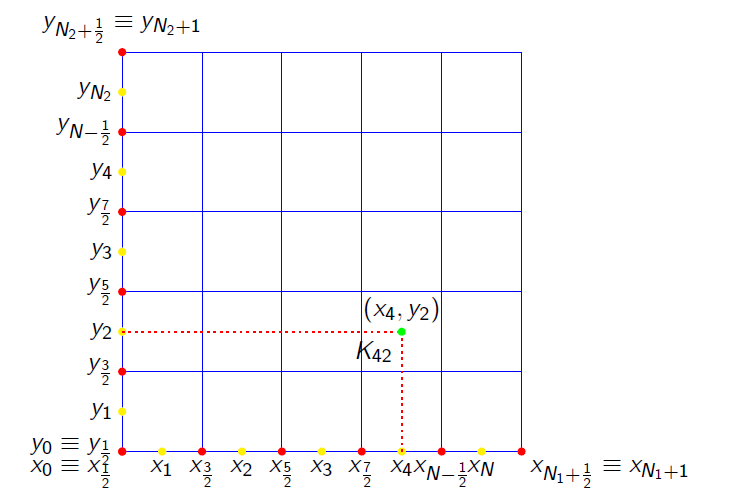
\includegraphics[scale=0.35]{1}
\end{center}
\end{block}
\end{frame}

\begin{frame}\frametitle{Mesh}
\begin{block}{Mesh}
Consider $\Omega = (0,1) \times (0,1)$ . On interval [0,1] we make two partition $(x_{i+\frac{1}{2}})_{i\in \overline{0,N_1}}$,$(y_{j+\frac{1}{2}})_{j\in \overline{0,N_2}}$ s.t
$$0=x_{\frac{1}{2}}< x_{\frac{3}{2}} < ... < x_{N_1-\frac{1}{2}} < x_{N_1+\frac{1}{2}} =1 $$ 
$$0=y_{\frac{1}{2}}< y_{\frac{3}{2}} < ... < y_{N_1-\frac{1}{2}} < y_{N_1+\frac{1}{2}} =1 $$ 
Let $\tau=(T_{ij})_{i\in \overline{1,N_1},j\in \overline{1,N_2}}$ be an admissible mesh of $(0,1) \times (0,1)$ s.t
$$T_{ij}=[x_{i-\frac{1}{2}},x_{i+\frac{1}{2}}] \times [y_{i-\frac{1}{2}},y_{i+\frac{1}{2}}]$$
$T_{ij}$ is called a control volume of $\tau$ . The point $(x_{i+\frac{1}{2})},y_{j+\frac{1}{2}})$ are called mesh points.
\end{block}
\end{frame}

\begin{frame}\frametitle{Mesh}
\begin{block}{Mesh}
Choosing the sequences $(x_{i})_{i\in \overline{0,N_1+1}}$,$(y_{j})_{j\in \overline{0,N_2+1}}$ s.t
$$x_0=x_{\frac{1}{2}},x_i= \frac{1}{2}(x_{i-\frac{1}{2}}+x_{i+\frac{1}{2}}) , x_{N_1+1} = x_{N_1+\frac{1}{2}} =1 $$ 
$$y_0=y_{\frac{1}{2}},y_j= \frac{1}{2}(y_{j-\frac{1}{2}}+y_{j+\frac{1}{2}}) , y_{N_2+1} = y_{N_2+\frac{1}{2}} =1 $$ 
The point $(x_i,y_J)$ is called a control point of control volume $T_{ij}$ \\
Let
$$h_i=|x_{i+\frac{1}{2})}-x_{i-\frac{1}{2})}|, \quad k_j=|y_{j+\frac{1}{2})}-y_{j-\frac{1}{2})}| \quad \forall i\in \overline{1,N_1} ,j\in \overline{1,N_2}$$ 
$$h_{i+\frac{1}{2}}=|x_{i+1)}-x_{i}|, \quad k_{j+\frac{1}{2}}=|y_{j+1}-y_{j}| \quad \forall i\in \overline{0,N_1} ,j\in \overline{0,N_2}$$ 
Then the area of control volume $T_{ij}$=$h_ik_j$, $h=max\left \{ h_i,k_j \right \}$ is the mesh size
\end{block}
\end{frame}

\begin{frame}{Preliminary}
\begin{block}{Formula}
throughout this presentation we use the following formula : 
\begin{align}
\int_a^bf(x)dx=\frac{b-a}{2}(f(a)+f(b)) + error \label{2.1}
\end{align}
and 
\begin{equation*}
\frac{1}{|T_{ij}|}\int_{T_{ij}}f=\frac{1}{4}\left ( f(x_i,y_{j-\frac{1}{2}})+f(x_i,y_{j+\frac{1}{2}})+f(x_{i-\frac{1}{2}},y_{j})+f(x_{i+\frac{1}{2}},y_{j})  \right ) +error
\end{equation*}
\end{block}
\end{frame}

\begin{frame}\frametitle{Scheme}
\begin{block}{Scheme}
The finite volume scheme is found by integrating \ref{1.1} over each control volume $T_{ij}$ , which gives
\begin{equation}
\frac{1}{|T_{ij}|}\int_{T_{ij}}-\Delta udxdy+\frac{1}{|T_{ij}|}\int_{T_{ij}} \frac{\partial p}{\partial x}dxdy=\frac{1}{|T_{ij}|}\int_{T_{ij}} fdxdy 
\end{equation}
The first term in (2.3) is exactly what we have learn in our course so we just need consider the second term in LHS
\end{block}
\end{frame}
\begin{frame}\frametitle{Scheme}
Using formula \ref{2.1} we get : 
\begin{align*}
\frac{1}{|T_{ij}|}\int_{T_{ij}} \frac{\partial p}{\partial x}dxdy =& \frac{1}{|T_{ij}|} \int_{y_{j-\frac{1}{2}}}^{y_{j+\frac{1}{2}}} \int_{x_{i-\frac{1}{2}}}^{x_{i+\frac{1}{2}}} \frac{\partial p}{\partial x}dxdy  \\
&= \frac{1}{|T_{ij}|} \left ( \int_{y_{j-\frac{1}{2}}}^{y_{j+\frac{1}{2}}} p(x_{i+\frac{1}{2}},y)-p(x_{i-\frac{1}{2}},y)dy \right ) \\
& = \frac{1}{h_{i}} \left(p(x_{i+\frac{1}{2}},y_{j})-p(x_{i-\frac{1}{2}},y_{j})\right) 
\end{align*}
\end{frame}
\begin{frame}\frametitle{Scheme}
We will consider three following cases: \\
Case 1: if $i \neq 1 $ and $ i \neq N $
\begin{align*}
\frac{1}{|T_{ij}|}\int_{T_{ij}} \frac{\partial p}{\partial x}dxdy &= \frac{1}{h_{i}}\left(\frac{p_{i+1,j}+p_{i,j}}{2}-\frac{p_{i,j}+p_{i-1,j}}{2}\right) \\
& = \frac{1}{2h_{i}}(p_{i+1,j}-p_{i-1,j})
\end{align*} 
Case 2: if $i = 1 $ 
\begin{align*}
\frac{1}{|T_{ij}|}\int_{T_{ij}} \frac{\partial p}{\partial x}dxdy &= \frac{1}{h_{i}}\left(\frac{p_{i+1,j}+p_{i,j}}{2}-p_{i,j}\right) \\
& = \frac{1}{2h_{i}}(p_{i+1,j}-p_{i,j})
\end{align*}
Case 3: if $i = N $
\begin{align*}
\frac{1}{|T_{ij}|}\int_{T_{ij}} \frac{\partial p}{\partial x}dxdy &= \frac{1}{h_{i}}\left(p_{i,j}-\frac{p_{i,j}+p_{i-1,j}}{2}\right) \\
& = \frac{1}{2h_{i}}(p_{i,j}-p_{i-1,j})
\end{align*}
\end{frame}
\begin{frame} \frametitle{Scheme}
\begin{block}{Scheme}
At cell (i,j) for $i \in [1,N_1]$ and $j\in [1,N_2]$
\begin{align*}
-a_iu_{i-1,j}-b_iu_{i+1,j}-c_ju_{i,j-1}-d_ju_{i,j+1}+s_{i,j}u_{i,j} \\ 
+\frac{1}{2h_{i}} (\epsilon_{i}p_{i-1,j} + \xi_{i}p_{i,j} + \eta_{i}p_{i+1,j})
 =f_{i,j}
\end{align*} 
\end{block}
where 
$$a_i=\frac{1}{h_ih_{i-\frac{1}{2}}},b_i=\frac{1}{h_ih_{i+\frac{1}{2}}}$$
$$c_j=\frac{1}{k_jk_{i-\frac{1}{2}}},d_j=\frac{1}{k_jk_{j+\frac{1}{2}}}$$
$$s_{i,j}=a_i+b_i+c_j+d_j$$
\end{frame}

\begin{frame}\frametitle{Scheme}
$$\epsilon(i)=\begin{cases}
-1 & \textbf{if} i \neq 1 \\
0 & \textbf{if}  i = 1
\end{cases}$$
$$\xi_{i}=\begin{cases}
-1 & \textbf{if} i = 1 \\
1 & \textbf{if}  i = N \\
0 & \textbf{if} i \neq 1,N
\end{cases}$$
$$\eta(i)=\begin{cases}
1 & \textbf{if} i \neq N \\
0 & \textbf{if}  i = N
\end{cases}$$
\end{frame}

\begin{frame}\frametitle{Scheme}
absolutely similar we get :
\begin{block}{Scheme}
At cell (i,j) for $i \in [1,N_1]$ and $j\in [1,N_2]$
\begin{align*}
-a_iv_{i-1,j}-b_iv_{i+1,j}-c_jv_{i,j-1}-d_jv_{i,j+1}+s_{i,j}v_{i,j} \\
+\frac{1}{2h_{i}} \left(\epsilon_{j}p_{i,j-1} + \xi_{j}p_{i,j} + \eta_{j}p_{i,j+1}\right)
 =f_{i,j}
\end{align*}   
\end{block}
\end{frame}

\begin{frame}\frametitle{Scheme}
 we now consider the equations :
\begin{block}{Scheme}
\begin{align*}
 \frac{\partial u}{\partial x}+& \frac{\partial v}{\partial y} = 0 \quad in \quad \Omega 
\end{align*}   
Intergrate over each control volume $T_{ij}$ which gives : 
\begin{align*}
\frac{1}{|T_{ij}|}\int_{T_{ij}} \frac{\partial u}{\partial x}+& \frac{\partial v}{\partial y} = 0
\end{align*}   
\end{block}
\end{frame}
\begin{frame}\frametitle{Scheme}
similarly when we doing with p we have : 
\begin{block}{Scheme}
\begin{align*}
\frac{u_{i+1,j}+u_{i,j}}{2h_{i}}-\frac{u_{i,j}+u_{i-1,j}}{2h_{i}}+\frac{v_{i,j+1}+v_{i,j}}{2k_{j}}-\frac{v_{i,j}+v_{i,j-1}}{2k_{j}}=0
\end{align*}   
\end{block}
\end{frame}
\begin{frame}\frametitle{Scheme}
In other word, 
\begin{block}{Scheme}
\begin{align*}
\frac{1}{2h_{i}}(\epsilon_{i}u_{i-1,j}+\xi_{i}u_{i,j}+\eta_{i}u_{i+1,j})+\frac{1}{2k_{j}}(\epsilon_{j}v_{i,j-1}+\xi_{j}v_{i,j}+\eta_{j}v_{i,j+1})=0
\end{align*}   
\end{block}
\end{frame}
\begin{frame}\frametitle{Matrix form}
\begin{align*}
K=\begin{bmatrix}
A & 0 & B\\ 
0 & A & D\\ 
B^T & D^T & 0 
\end{bmatrix}
\end{align*}  
where A is exactly in our course 
\begin{align*}
B=\frac{-1}{2h} \begin{bmatrix}
-1 & 1 &  &  &  & \\ 
-1 & 0 & 1 &  &  & \\ 
 & -1 & 0 & 1 &  & \\ 
 &  &  & ... &  & \\ 
 &  &  & -1 & 0 & 1\\ 
 &  &  &  & -1 & 1
\end{bmatrix}
\end{align*}
\end{frame}

\begin{frame}\frametitle{Matrix form}
\begin{align*}
D=\frac{-1}{2h} \begin{bmatrix}
-I & I &  &  &  & \\ 
-I & 0 & I &  &  & \\ 
 & -I & 0 & I &  & \\ 
 &  &  & ... &  & \\ 
 &  &  & -I & 0 & I\\ 
 &  &  &  & -I & I 
\end{bmatrix}
\end{align*} 
\end{frame}

\begin{frame}\frametitle{Matrix form}
\begin{align*}
KU=F
\end{align*} 
where 
\begin{align*}
F=[F_1, F_2, 0],U=[u,v,p]
\end{align*}

\end{frame}

\section{Experiemnt Test and Error}

\begin{frame}\frametitle{Experiment test}
Experiment Test we set up with the following system of equation 

\begin{align*}
u=(1-cos(2\pi x))sin(2 \pi y) \\
v=-(1-cos(2\pi y))sin(2 \pi x) \\
p=xy+x+y+x^3y^2-\frac{4}{3}
\end{align*}
\end{frame}
\begin{frame}\frametitle{Experiment test}
\begin{center}
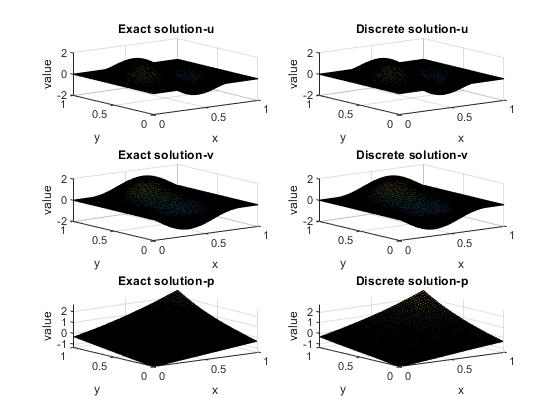
\includegraphics[scale=0.45]{2}
\end{center}
\end{frame}
\begin{frame}\frametitle{Experiment test}
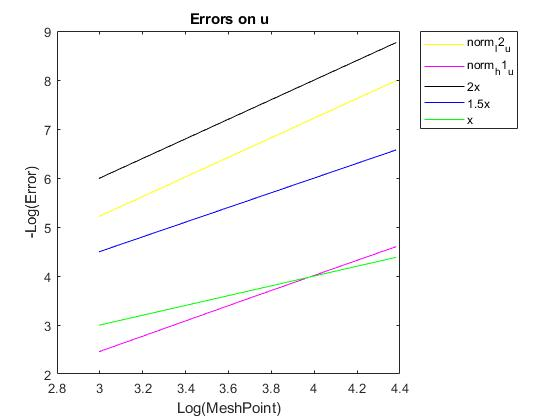
\includegraphics[scale=0.5]{3}
\end{frame}
\begin{frame}\frametitle{Experiment test}
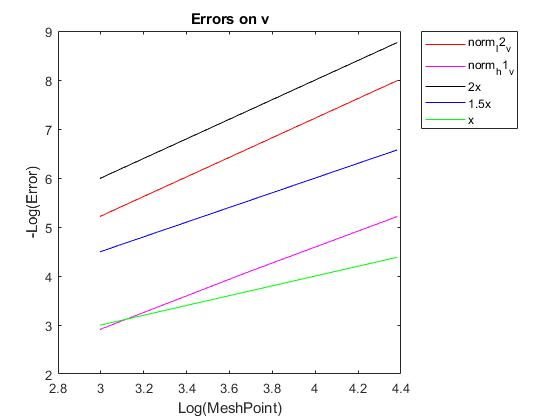
\includegraphics[scale=0.5]{4}
\end{frame}
\begin{frame}\frametitle{Experiment test}
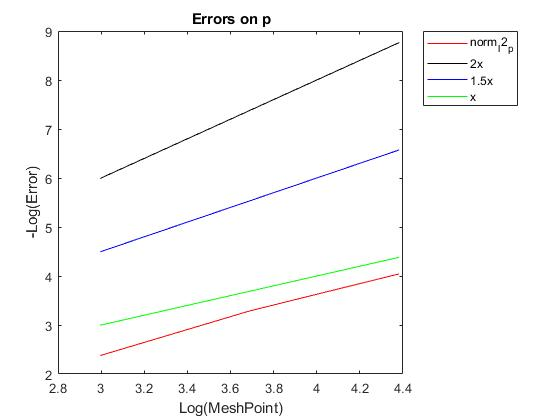
\includegraphics[scale=0.5]{5}
\end{frame}
\begin{frame}\frametitle{Error}
\begin{block}{Error}
\begin{tabular}{|l||c||c||c|}
\hline 
number of elements  & 20 & 40 & 80  \\ 
\hline 
Error of $L_2$ norm on u  & 0.0054  &0.0014 & 0.0003  \\
\hline
Error of $H_0^1$ norm on u  & 0.0859 & 0.0292 & 0.0101  \\
\hline
Error of $L_2$ norm on v  & 0.0054  &0.0014 & 0.0003  \\
\hline
Error of $H_0^1$ norm on v  & 0.0545 & 0.0168 & 0.0054  \\
\hline
Error of $L_2$ norm on p  & 0.0929  &0.0374 & 0.0175  \\
\hline
\end{tabular}
\end{block}
\end{frame}
\begin{frame}\frametitle{Experiment test}
One more example ! 
\begin{align*}
u=(1-cos(2\pi x))sin(2 \pi y) \\
v=-(1-cos(2\pi y))sin(2 \pi x) \\
p=-2\pi(cos(2\pi x)-cos(2\pi y)) 
\end{align*}
\end{frame}
\begin{frame}\frametitle{Experiment test}
\begin{center}
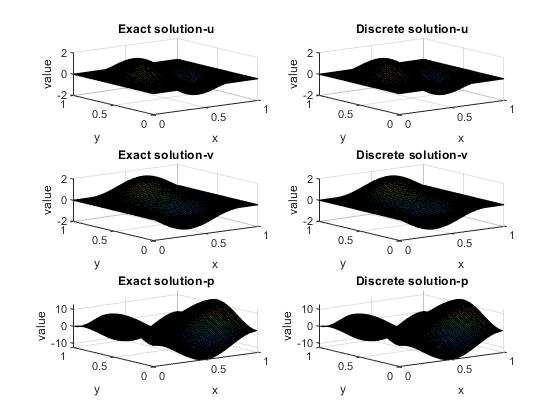
\includegraphics[scale=0.45]{6}
\end{center}
\end{frame}
\begin{frame}\frametitle{Experiment test}
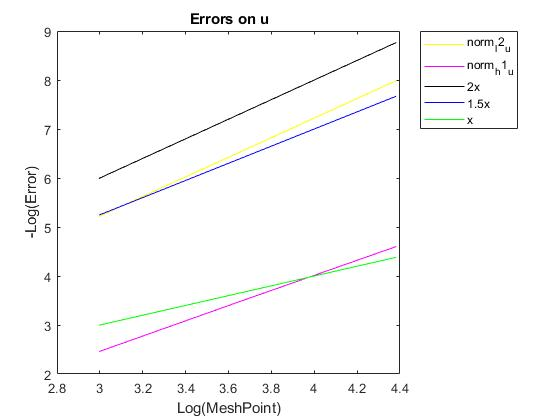
\includegraphics[scale=0.5]{7}
\end{frame}
\begin{frame}\frametitle{Experiment test}
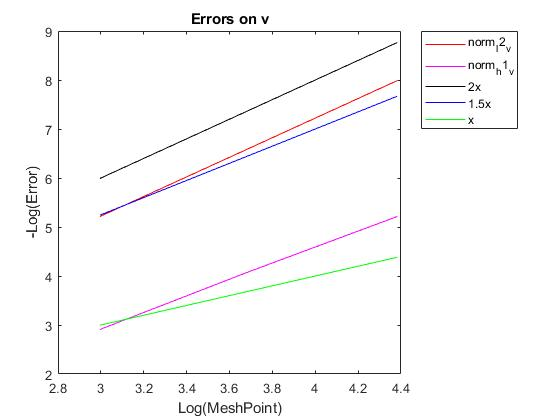
\includegraphics[scale=0.5]{8}
\end{frame}
\begin{frame}\frametitle{Experiment test}
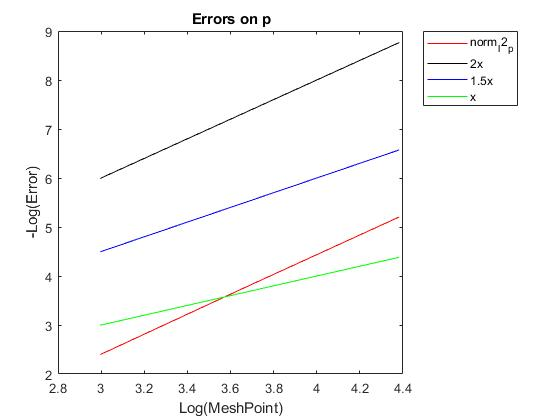
\includegraphics[scale=0.5]{9}
\end{frame}
\begin{frame}\frametitle{Error}
\begin{block}{Error}
\begin{tabular}{|l||c||c||c|}
\hline 
number of elements  & 20 & 40 & 80  \\ 
\hline 
Error of $L_2$ norm on u  & 0.0054  &0.0014 & 0.0003  \\
\hline
Error of $H_0^1$ norm on u  & 0.0857 & 0.0292 & 0.0100  \\
\hline
Error of $L_2$ norm on v  & 0.0054  &0.0014 & 0.0003  \\
\hline
Error of $H_0^1$ norm on v  & 0.0545 & 0.0168 & 0.0054  \\
\hline
Error of $L_2$ norm on p  & 0.0054  &0.0014 & 0.0003  \\
\hline
\end{tabular}
\end{block}
\end{frame}

\begin{frame}\frametitle{Solved by Uzawa method}

\begin{align*}
u=(1-cos(2\pi x))sin(2 \pi y) \\
v=-(1-cos(2\pi y))sin(2 \pi x) \\
p=xy+x+y+x^3y^2-\frac{4}{3}
\end{align*}
\end{frame}
\begin{frame}\frametitle{Solved by Uzawa method}
\begin{center}
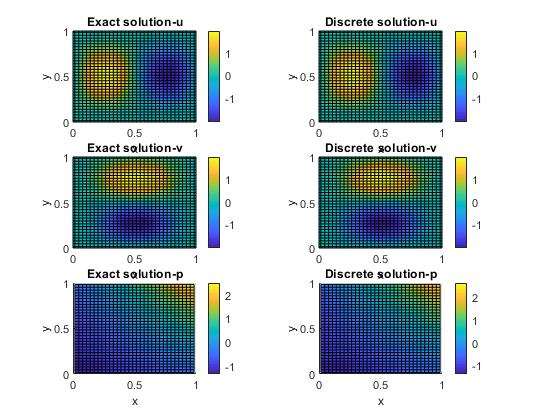
\includegraphics[scale=0.45]{10}
\end{center}
\end{frame}
\begin{frame}\frametitle{Solved by Uzawa method}
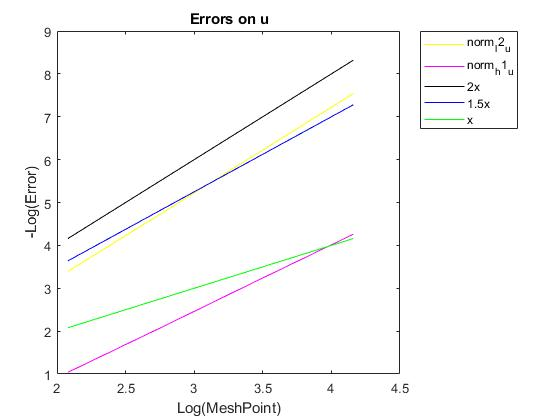
\includegraphics[scale=0.5]{11}
\end{frame}
\begin{frame}\frametitle{Solved by Uzawa method}
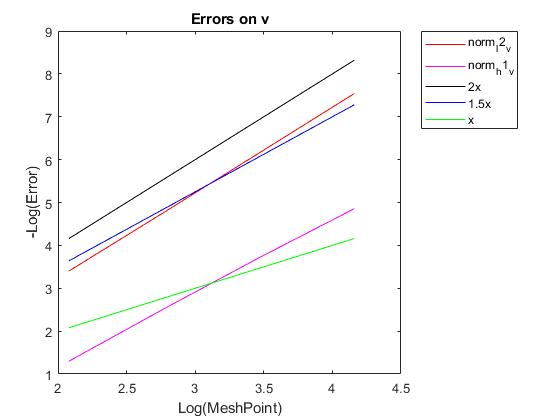
\includegraphics[scale=0.5]{12}
\end{frame}
\begin{frame}\frametitle{Solved by Uzawa method}
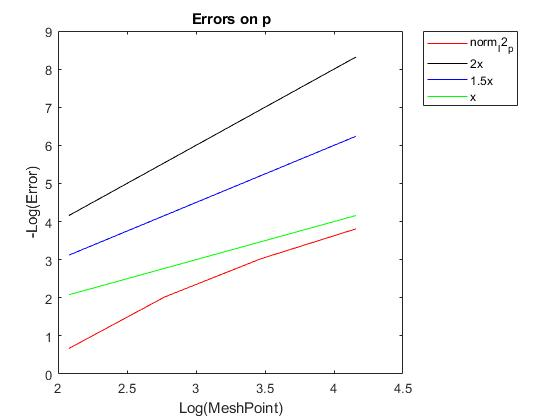
\includegraphics[scale=0.5]{13}
\end{frame}
\begin{frame}\frametitle{Error}
\begin{block}{Error}
\begin{tabular}{|l||c||c||c||c|}
\hline 
number of elements  & 8 & 16 & 32 & 64  \\ 
\hline 
Error of $L_2$ norm on u  & 0.0336  &0.0085 & 0.0021 & 0.0005  \\
\hline
Error of $H_0^1$ norm on u  & 0.3536 & 0.1218 & 0.0413 & 0.0141 \\
\hline
Error of $L_2$ norm on v  & 0.0333  &0.0085 & 0.0021 & 0.0005  \\
\hline
Error of $H_0^1$ norm on v  & 0.2729 & 0.0803 & 0.0244 & 0.0078  \\
\hline
Error of $L_2$ norm on p  & 0.5112  &0.1325 & 0.0489 & 0.0222  \\
\hline
\end{tabular}
\end{block}
\end{frame}
\begin{frame}\frametitle{Solved by Uzawa method}
One more example ! 
\begin{align*}
u=(1-cos(2\pi x))sin(2 \pi y) \\
v=-(1-cos(2\pi y))sin(2 \pi x) \\
p=-2\pi(cos(2\pi x)-cos(2\pi y)) 
\end{align*}
\end{frame}
\begin{frame}\frametitle{Solved by Uzawa method}
\begin{center}
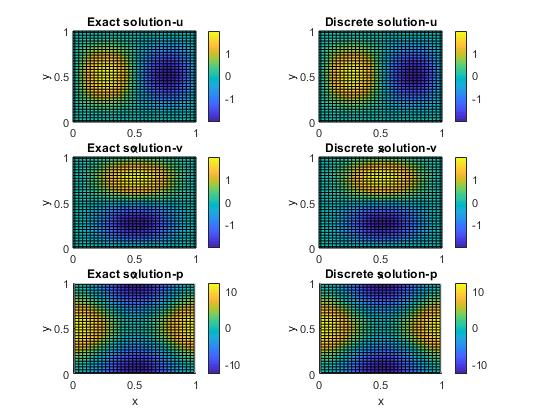
\includegraphics[scale=0.45]{14}
\end{center}
\end{frame}
\begin{frame}\frametitle{Solved by Uzawa method}
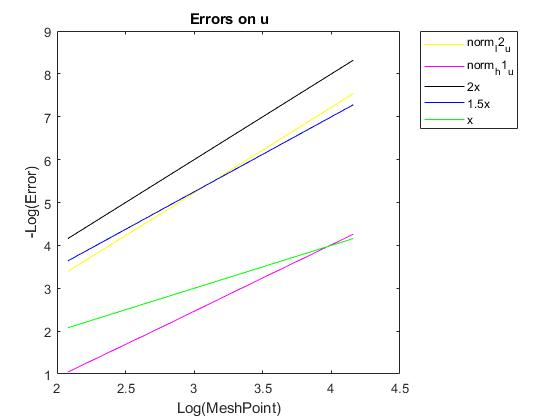
\includegraphics[scale=0.5]{15}
\end{frame}
\begin{frame}\frametitle{Solved by Uzawa method}
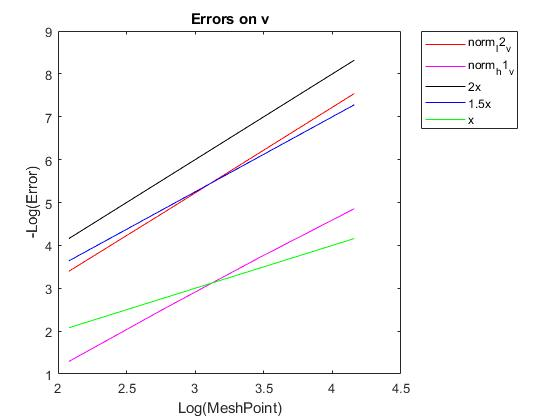
\includegraphics[scale=0.5]{16}
\end{frame}
\begin{frame}\frametitle{Solved by Uzawa method}
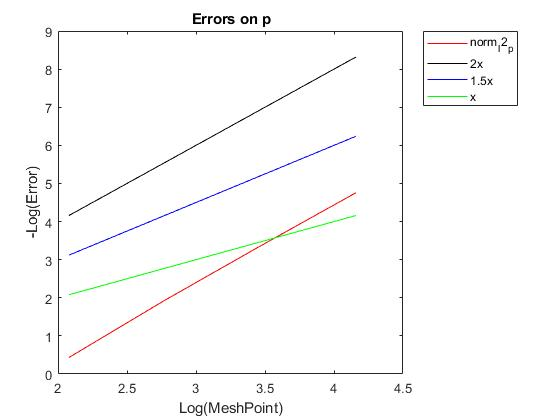
\includegraphics[scale=0.5]{17}
\end{frame}

\begin{frame}\frametitle{Error}
\begin{block}{Error}
\begin{tabular}{|l||c||c||c||c|}
\hline 
number of elements  & 8 & 16 & 32 & 64  \\ 
\hline 
Error of $L_2$ norm on u  & 0.0335  &0.0085 & 0.0021 & 0.0005  \\
\hline
Error of $H_0^1$ norm on u  & 0.3510 & 0.1214 & 0.0412 & 0.0141  \\
\hline
Error of $L_2$ norm on v  & 0.0335  &0.0085 & 0.0021 & 0.0005  \\
\hline
Error of $H_0^1$ norm on v  & 0.2745 & 0.0804 & 0.0244 & 0.0078  \\
\hline
Error of $L_2$ norm on p  & 0.6482  &0.1449 & 0.0348 & 0.0086  \\
\hline
\end{tabular}
we can see that when we solved by uzawa , order convergence of p is increase ! 
\end{block}
\end{frame}

\begin{frame}\frametitle{Uniqueness of solution}
we have that 
\begin{align*}
\begin{pmatrix}
A & B\\ 
B^T & 
\end{pmatrix}\begin{pmatrix}
x_1\\ 
x_2
\end{pmatrix}=\begin{pmatrix}
f_1\\ 
f_2
\end{pmatrix}
\end{align*}
in order to prove that it is suffice to prove if $f_1,f_2=0$ then $x_1,x_2=0$ , indeed
\begin{align*}
\left\{\begin{matrix}
Ax_1+Bx_2=0 \\ 
B^Tx_2=0
\end{matrix}\right.
\end{align*}
\end{frame}
\begin{frame}\frametitle{Uniqueness of solution}
Or
Multiplying the first row by $B^TA^{-1}$ and subtracting from the second row yields 
$$-B^TA^{-1}Bx_2=0$$ 
we have that $-B^TA^{-1}B$ is symmetric positive-definite we conclude that $x_2=0$ or $Ax_1=0$ since A is invertible we conclude that $x_1=0$
\end{frame}
\begin{frame}
\begin{center}
\huge{ \textbf{Thanks For Watching}}
\end{center}
 \end{frame}
\end{document}




